% **************************************************
% Document Class Definition
% **************************************************
\documentclass[%
    paper=A4,               % paper size --> A4 is default in Germany
    twoside=true,           % onesite or twoside printing
    openright,              % doublepage cleaning ends up right side
    parskip=half,           % spacing value / method for paragraphs
    chapterprefix=true,     % prefix for chapter marks
    11pt,                   % font size
    headings=normal,        % size of headings
    bibliography=totoc,     % include bib in toc
    listof=totoc,           % include listof entries in toc
    titlepage=on,           % own page for each title page
    captions=tableabove,    % display table captions above the float env
    chapterprefix=false,    % do not display a prefix for chapters
    appendixprefix=false,    % but display a prefix for appendix chapter
    draft=false,            % value for draft version
]{scrreprt}%


% **************************************************
% Setup YOUR thesis document in this file !
% **************************************************
% !TEX root = thesis.tex


% **************************************************
% Files' Character Encoding
% **************************************************
\PassOptionsToPackage{utf8}{inputenc}
\usepackage{inputenc}


% **************************************************
% Information and Commands for Reuse
% **************************************************
\newcommand{\thesisTitle}{A Practical Analysis of UEFI Threats Against Windows~11}
\newcommand{\thesisName}{Joshua Machauer}
\newcommand{\thesisSubject}{Bachelor's Thesis}
\newcommand{\thesisDate}{December 25, 2022}
\newcommand{\thesisDateGerman}{25. Dezember 2022}
\newcommand{\thesisVersion}{Draft 1.0}

\newcommand{\thesisFirstReviewer}{Prof. Dr. Jean-Pierre Seifert}
\newcommand{\thesisFirstReviewerUniversity}{\protect{Technische Universität Berlin}}
\newcommand{\thesisFirstReviewerDepartment}{Electrical Engineering and Computer Science}

\newcommand{\thesisSecondReviewer}{Prof. Dr. Stefan Schmid}
\newcommand{\thesisSecondReviewerUniversity}{\protect{Technische Universität Berlin}}
\newcommand{\thesisSecondReviewerDepartment}{Electrical Engineering and Computer Science}

\newcommand{\thesisFirstSupervisor}{Hans Niklas Jacob}
\newcommand{\thesisSecondSupervisor}{Christian Werling}

\newcommand{\thesisUniversity}{\protect{Technische Universität Berlin}}
\newcommand{\thesisUniversityDepartment}{Electrical Engineering and Computer Science}
\newcommand{\thesisUniversityInstitute}{Institute of Software Engineering and Theoretical Computer Science}
\newcommand{\thesisUniversityGroup}{Security in Telecommunications (SecT)}
\newcommand{\thesisUniversityCity}{Berlin}
\newcommand{\thesisUniversityStreetAddress}{Ernst-Reuter-Platz 7}
\newcommand{\thesisUniversityPostalCode}{10587}



% **************************************************
% Debug LaTeX Information
% **************************************************
%\listfiles


% **************************************************
% Load and Configure Packages
% **************************************************
\usepackage[english]{babel} % babel system, adjust the language of the content
\usepackage{acronym}[printonlyused]
\PassOptionsToPackage{% setup clean thesis style
    figuresep=colon,%
    hangfigurecaption=false,%
    hangsection=true,%
    hangsubsection=true,%
    sansserif=false,%
    configurelistings=true,%
    colorize=full,%
    colortheme=bluemagenta,%
    configurebiblatex=true,%
    bibsys=biber,%
    bibfile=bib-refs,%
    %bibstyle=alphabetic,%			-> citations with alphabetic enumeration
    %bibstyle=numeric-comp,%		-> citations with numeric compressed numeric sorting
    bibstyle=ieee-alphabetic,%		-> citations with IEEE transactions-like style with numeric labels
    %bibsorting=nty,% 
    bibsorting=none,%				-> sorted in the order of the citations from start to finish
}{cleanthesis}
\usepackage{cleanthesis}

\hypersetup{% setup the hyperref-package options
    pdftitle={\thesisTitle},    %   - title (PDF meta)
    pdfsubject={\thesisSubject},%   - subject (PDF meta)
    pdfauthor={\thesisName},    %   - author (PDF meta)
    plainpages=false,           %   -
    colorlinks=false,           %   - colorize links?
    pdfborder={0 0 0},          %   -
    breaklinks=true,            %   - allow line break inside links
    bookmarksnumbered=true,     %
    bookmarksopen=true          %
}


\graphicspath{{./images/}{./figures/}}
\usepackage{svg}

\usepackage{multirow}
\usepackage[shortcuts]{extdash}

\usepackage{textcmds}



% **************************************************
% Document CONTENT
% **************************************************
\begin{document}

% uncomment the following command to fill up pages with
% whitespace instead of aligning the first and last lines
% of a page (see \raggedbottom vs. \flushbottom)
%\raggedbottom

% --------------------------
% rename document parts
% --------------------------
\renewcaptionname{english}{\figurename}{Fig.}
\renewcaptionname{english}{\tablename}{Tab.}

% --------------------------
% Front matter
% --------------------------
\pagenumbering{roman}			% roman page numbing (invisible for empty page style)
\pagestyle{empty}				% no header or footers
% !TEX root = ../thesis.tex
%
% ------------------------------------  --> cover title page
\begin{titlepage}
	\pdfbookmark[0]{Cover}{Cover}
	\flushright
	\hfill
	\vfill
	{\LARGE\thesisTitle \par}
	\rule[5pt]{\textwidth}{.4pt} \par
	{\Large\thesisName}
	\vfill
	\textit{\large\thesisDate} \\
	Version: \thesisVersion
\end{titlepage}


% ------------------------------------  --> main title page
\begin{titlepage}
	\pdfbookmark[0]{Titlepage}{Titlepage}
	\tgherosfont
	\centering

	{\Large \thesisUniversity} \\[4mm]
	
\includegraphics[width=6cm]{gfx/Clean-Thesis-Logo} \\[2mm]
	\textsf{\thesisUniversityDepartment} \\
	\textsf{\thesisUniversityInstitute} \\
	\textsf{\thesisUniversityGroup} \\

	\vfill
	{\large \thesisSubject} \\[5mm]
	{\LARGE \color{ctcolortitle}\textbf{\thesisTitle} \\[10mm]}
	{\Large \thesisName} \\

	\vfill
	\begin{minipage}[t]{.27\textwidth}
		\raggedleft
		\textit{1. Reviewer}
	\end{minipage}
	\hspace*{15pt}
	\begin{minipage}[t]{.65\textwidth}
		{\Large \thesisFirstReviewer} \\
		{\small \thesisFirstReviewerDepartment} \\[-1mm]
		{\small \thesisFirstReviewerUniversity}
	\end{minipage} \\[5mm]
	\begin{minipage}[t]{.27\textwidth}
		\raggedleft
		\textit{2. Reviewer}
	\end{minipage}
	\hspace*{15pt}
	\begin{minipage}[t]{.65\textwidth}
		{\Large \thesisSecondReviewer} \\
		{\small \thesisSecondReviewerDepartment} \\[-1mm]
		{\small \thesisSecondReviewerUniversity}
	\end{minipage} \\[10mm]
	\begin{minipage}[t]{.27\textwidth}
		\raggedleft
		\textit{Supervisors}
	\end{minipage}
	\hspace*{15pt}
	\begin{minipage}[t]{.65\textwidth}
		\thesisFirstSupervisor\ and \thesisSecondSupervisor
	\end{minipage} \\[10mm]

	\thesisDate \\

\end{titlepage}


% ------------------------------------  --> lower title back for single page layout
\hfill
\vfill
{
	\small
	\textbf{\thesisName} \\
	\textit{\thesisTitle} \\
	\thesisSubject, \thesisDate \\
	Reviewers: \thesisFirstReviewer\ and \thesisSecondReviewer \\
	Supervisors: \thesisFirstSupervisor\ and \thesisSecondSupervisor \\[1.5em]
	\textbf{\thesisUniversity} \\
	\textit{\thesisUniversityGroup} \\
	\thesisUniversityInstitute \\
	\thesisUniversityDepartment \\
	\thesisUniversityStreetAddress \\
	\thesisUniversityPostalCode\ \thesisUniversityCity
}
		% INCLUDE: all titlepages
\cleardoublepage

% !TEX root = ../thesis.tex
%
%************************************************
% Declaration
%************************************************
\pdfbookmark[0]{Selbst\"andigkeitserkl\"arung}{Selbst\"andigkeitserkl\"arung}
\chapter*{Selbst\"andigkeitserkl\"arung}
\label{sec:declaration}
\thispagestyle{empty}

Hiermit erkl\"are ich, dass ich die vorliegende Arbeit selbstst\"andig und eigenh\"andig sowie ohne
unerlaubte fremde Hilfe und ausschlie\ss{}lich unter Verwendung der aufgef\"uhrten Quellen und
Hilfsmittel angefertigt habe.

\bigskip

\noindent\textit{\thesisUniversityCity, den \thesisDateGerman}

\smallskip

\begin{flushright}
	\begin{minipage}{5cm}
		\rule{\textwidth}{1pt}
		\centering\thesisName
	\end{minipage}
\end{flushright}

%*****************************************
%*****************************************
\cleardoublepage

\pagestyle{plain}				% display just page numbers
% !TEX root = ../thesis.tex

% http://williamstallings.com/Extras/Abstract.html
% https://www.enago.com/academy/abstract-versus-introduction-difference/

\pdfbookmark[0]{Abstract}{Abstract}
\addchap*{Abstract}
\label{sec:abstract}

% motivation
In Computer Security one of the most feared security threats is a rootkit, executing at the beginning of a computers boot chain, before the operating system and accompanying antivirus programs. With the widespread adaption of standardized UEFI firmware these threats have become less machine dependent and can now target a host of systems at once.
% problem statement
Past analyses about bootkits have been case studies of their appearances in the wild, this thesis instead aims to be a more practical approach by developing a bootkit and analyzing the challenges doing so.
% approach
We restrict our analysis by assuming an attacker has already gained read and write access to the BIOS image and is thus only facing security mechanisms involved during and with execution of the bootkit.
% results
Our bootkit was able to achieve elevated execution on Windows 11 by exploiting unrestricted hard drive access to edit Windows Registries, this was also possible on BitLocker encrypted hard drives by keylogging the Recovery Key.
% conclusions
UEFI makes it very easy for an attacker who has gained access to the System Firmware to leverage its powers and gain full control over the system.

\vspace*{20mm}

{\usekomafont{chapter}Abstract (different language)}
\label{sec:abstract-diff}

\blindtext
		% INCLUDE: the abstracts (english and german)
\cleardoublepage
%
% !TeX root = ../thesis.tex
%
\pdfbookmark[0]{Acknowledgement}{Acknowledgement}
\chapter*{Acknowledgement}
\label{sec:acknowledgement}
\thispagestyle{empty}


 % INCLUDE: acknowledgement
\cleardoublepage
%
\currentpdfbookmark{\contentsname}{toc}
\setcounter{tocdepth}{2}		% define depth of toc
\tableofcontents				% display table of contents
\cleardoublepage

% --------------------------
% Body matter
% --------------------------
\pagenumbering{arabic}			% arabic page numbering
\setcounter{page}{1}			% set page counter
\pagestyle{scrheadings}			% header and footer style

%\part{Example Part}
% !TeX root = ../thesis.tex

% https://www.enago.com/academy/abstract-versus-introduction-difference/
% https://www.student.unsw.edu.au/introductions
% https://www.scribbr.com/dissertation/introduction-structure/

\chapter{Introduction}


% what is UEFI
As the first piece of software that is run on your computer, UEFI holds an immense amount of responsibility during system initialization, attacks targeting your operating system from this environment are executed long before

what does it different than bios
this helps write platform independent code
uefi threats:
% definition of rootkit and bootkit
A rootkit is a collection of software designed to grant a threat actor control over a system, typically with malicious intend.
Rootkits set up a backdoor exploit and may deliver additional malware while leveraging their privileges to remain hidden.
There are different types of rootkits such as User Mode, Kernel Mode, Bootkits (bootloader rootkits), Hypervisor and Firmware rootkits.
\cite{crowdstrike, techtarget}
\TODO{consult abstract for similar definition, how easy uefi makes it to write hardware independent payload}
Firmware rootkits targets the software running during the boot process, which is responsible for the system initialization. This is done before the operating system is executed making them particularly hard to find, they are also persistent across operating system installation or hard drive replacements.
\cite{crowdstrike}


look at UEFI + threats against windows
danger of uefi infection
in recent years root and bootkits have popped up in the wild and been analysed
differences of root-/bootkits
reason about infection scenarios
we will discuss their commonalities
attack vectors:
- storage based
- memory based
implement a storage based ourselves
analyse security mechanism to prevent these attacks by attempting an attack itself
discuss security mechanisms we encounter
increasing security mechanisms
reflect their weaknesses
how to potentially evade them
- analyse countermeasures against UEFI threats
- Trusted Boot: KMCI from windows
- Secure Boot
- TPM
- Bitlocker
- firmware lock + signed capsule update
-



We start off introducing all background information necessary to understand this thesis in Chapter 2. With this knowledge we then look at analyses of previously discovered UEFI threats in Chapter 3. In Chapter 4 we start our practical approach by implementing a UEFI attack of our own to analyse security mechanism faced when attempting attacks from the UEFI environment. Afterwards we dicuss the impact of our findings as well as potential mitigation techniques in Chapter 5. Chapter 6 concludes ...

% !TEX root = ../../thesis.tex

\chapter{Background}

The following introduces the background information necessary to understand the employment of a \ac{UEFI} rootkit. This includes the general workings of the \acf{PI} and \ac{UEFI}, the \ac{UEFI} programming model and interface itself; as well as its security mechanisms. It is also necessary to understand our target's defenses, for this, we briefly describe the Window's security mechanisms faced when performing our attacks.

\section{Security Theory}

% !TeX root = ../../../thesis.tex

\section{\acs{UEFI}/\acs{PI}}
% what is it
\textcquote{uefi-spec-overview}{The \ac{UEFI} specifications define a new model for the interface between personal-computer \ac{OS} and \ac{PF}. \textelp{} Together, these provide a standard environment for booting an \ac{OS} and running pre-boot applications}.

UEFI is pure interface spec
\cite{beyond-bios}
% why does it exist
It was designed to replace the legacy \acl{BF} \ac{BIOS}, while also often offering a backwards compatible mode with the \acf{CSM}.
% what it defines
The specification is a pure interface specification thus merely states what interfaces and structures a \ac{PF} has to offer and what an \ac{OS} may use.
% what it doesn't define
how it is implemented by PF
what is used by OS
% what does it consist of
boot- and runttime service functions for the bootloader and os to call
datatables containing platform-related information
% what are its concrete goals
- complete solution describing all features and capabilities
- abstract interfaces to support a range of processors without the need for knowledge about underlying hardware for the bootloader
- sharable persistent storage for platform support code
security

\subsection{Boot Sequence}

% https://edk2-docs.gitbook.io/edk-ii-build-specification/2_design_discussion/23_boot_sequence

focus will be on dxe and transient system load

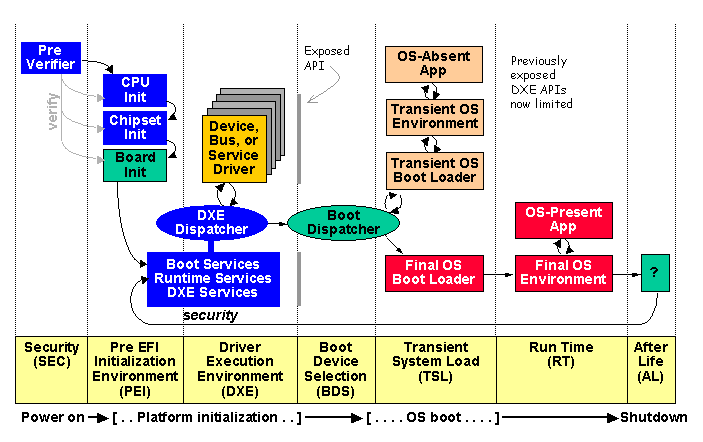
\includegraphics[width=\textwidth]{boot_sequence}


\begin{enumerate}
    \item{\acf{SEC}}

    % The SEC phase is the first phase in the UEFI boot process. It is specified in \cite[Vol 1, Section 13 ]{pi-spec}. Under its responsibilities fall setting up temporary memory used for the stack and the establishment of the system's root of trust which is a foundation for all secure operations. Inductive security designs rely on this root of trust to build a chain of trust by having a module verify the integrity of its subsequent module.
    ref to PSP

    inductive security design
    integrity of next module checked by the previous module

    handles all platform restart events
    applying power to system from unpowered state
    restarting from active state
    receiving exception conditions

    creates temporary memory store
    possibly CPU \ac{CAR}
    cache behaves as linear store of memory
    no evictions mode
    every memory access is a hit
    eviction not supported as main memory is not set up yet and would lead to platform failure


    final step
    Pass handoff information to the \ac{PEI} Foundation
    % what is the PEI foundation
    \begin{itemize}
        \item state of platform
        \item location and size of the \ac{BFV}
        \item location and size of the temporary RAM
        \item location and size of the stack
        \item optionally one or more \acp{HOB} via the \ac{SEC} \ac{HOB} Data \ac{PPI}
    \end{itemize}


    Part of this process is a so called \ac{HOB} with a function pointer to a procedure to verify PE modules.

    SEC Platform Information PPI
    information about the health of the processor

    SEC HOB Data PPI

    \item{\acf{PEI}}

    \begin{itemize}
        \item init permanent memory
        \item describe memory in \acp{HOB}
        \item describe \ac{FV} in \acp{HOB}
        \item pass control to \ac{DXE}
    \end{itemize}

    crisis recovery (what is this?)
    resuming from S3 sleep state
    linear array of RAM
    \ac{PEIM} provides a framework to allow vendors to supply separate initialization modules for
    each functionally distinct piece of system hardware that must be initialized prior to the DXE phase \cite{pi-spec}

    % design goals
    maintenance of chain of trust, protection against unauthorized updates to the PEI phase or modules
    authentication of the PEI Foundation and its modules
    provide core PEI module (PEI foundation) processor architecture independent, supports add-in moudles from vendors for processors, chipsets, RAM

    % what it does
    Locating, validating, and dispatching PEIMs
    Facilitating communication between PEIMs
    Providing handoff data to subsequent phases

    \item{\acf{DXE}}

    dxe core/foundation
    platform independent
    is implementation of UEFI
    UEFI Boot Services
    UEFI Runtime Services
    DXE Services

    dxe dispatcher
    discover drivers stored in firmware volumes and execute in proper order
    apriori file optionally in FV or depex of driver
    after dispatching all drivers in the dispatch queue hands control over to BDS

    dxe drivers
    init processor, chipset and platform
    produce arichtectural protocols and \ac{I/O} abstractions for consoles and boot devices

    % responsibilities
    initializing the processor, chipset, and platform components
    providing software abstractions for system services, console devices, and boot devices.

    \item{\acf{BDS}}

    DXE arichtectural protocol
    one function entry
    platform boot

    attempts to connect boot devices required to load the os
    discovers volumes containing new drivers
    calls DXE dispatcher
    doesnt return when successfully booting OS

    UEFI itself only specifies the NVRAM variables used in selecting boot options
    leaves the implementation of the menu system as value added implementation space \cite{uefi-spec}

    \cite{pi-spec}

    \begin{itemize}
        \item Initializing console devices
        \item Loading device drivers
        \item Attempting to load and execute boot selections
    \end{itemize}

    \item{\acf{TSL}}

    boottime and runtime services/driver
    bootloader
    \cite[13.3 System Partition]{uefi-spec}
    \cite[3.5.1.1]{uefi-spec}

    ExitBootServices()

    \item{\acf{RT}}

    runtime services/driver

    \item{\acf{AL}}

    hibernation
    sleep

\end{enumerate}

\subsection{\acs{UEFI}/\acs{PI} Firmware Images}

% https://edk2-docs.gitbook.io/edk-ii-build-specification/2_design_discussion/22_uefipi_firmware_images
\cite[Volume 3, 2.1]{pi-spec}

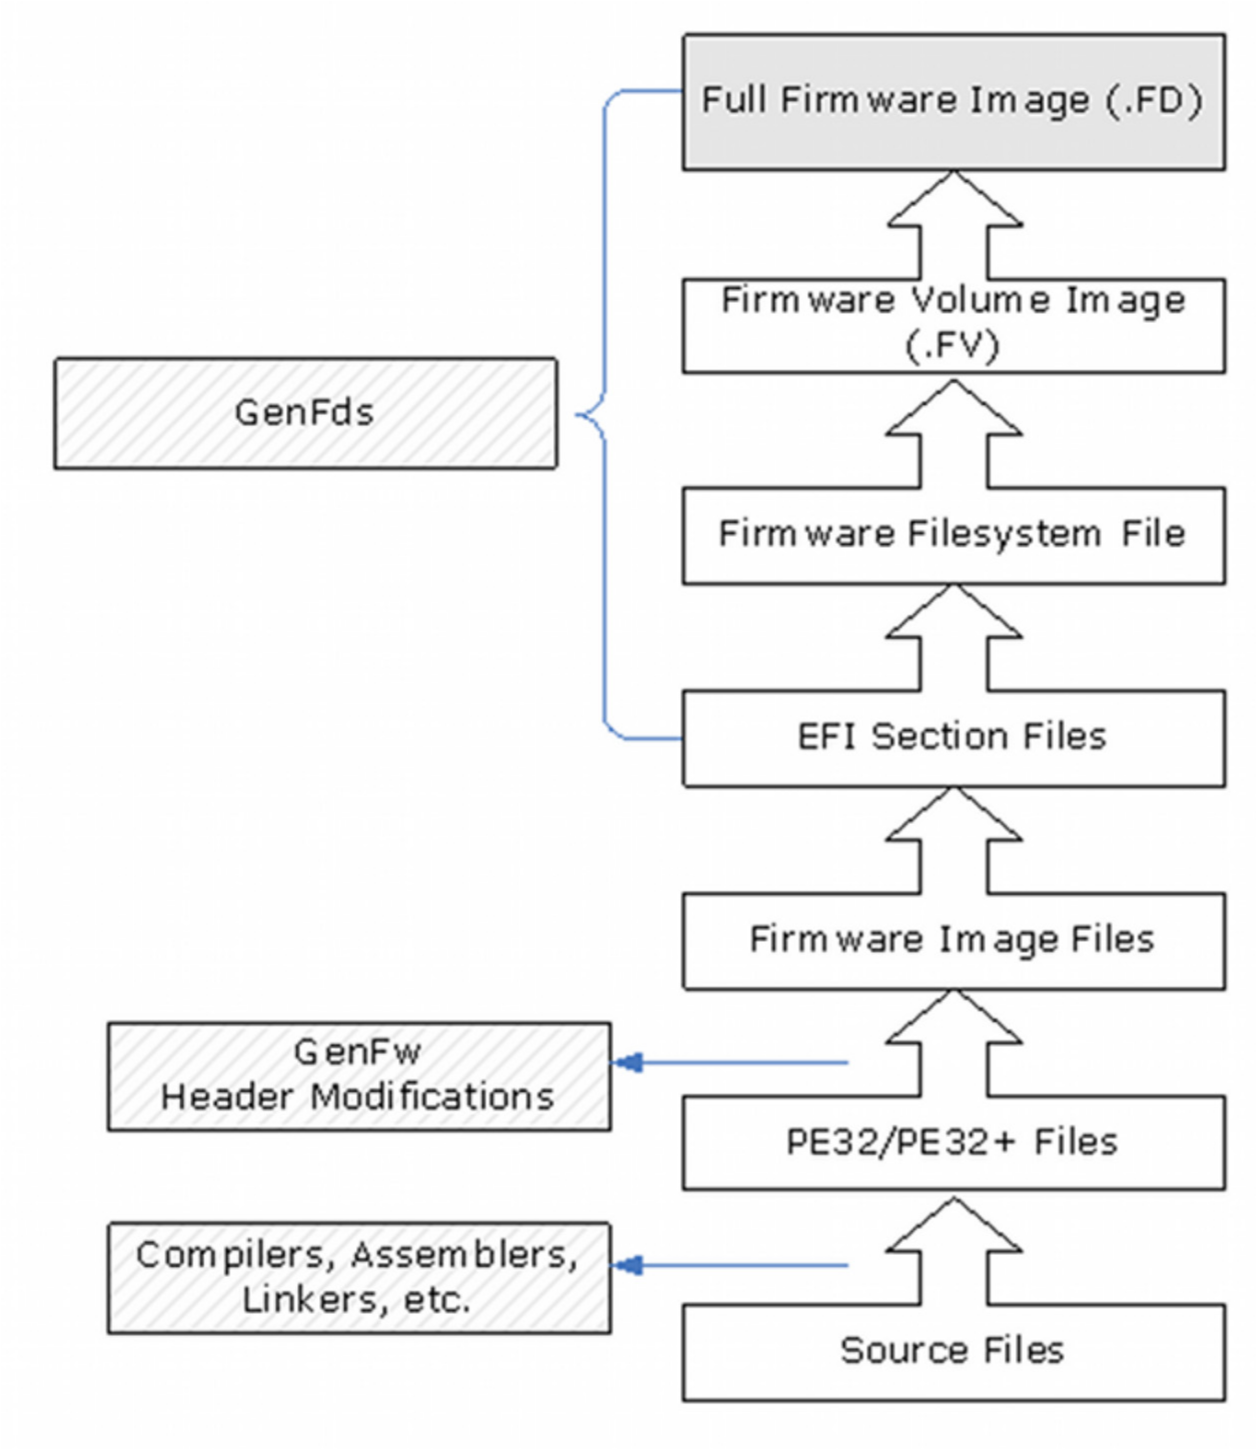
\includegraphics[width=\textwidth]{flash_device}
\ac{FD}
persistent
physical device
contains firmware code and/or data
typically flash
may be divided into smaller pieces to form multiple logical firmware devices
multiple physical firmware devices may be aggregated into one larger logical firmware device

\acf{FV}
logical device
organized into a file system
attributes such as
- size
- formatting
- read/write access

\acf{FFS}
organization of files and free space
no dierectory hierarchy
all files flat in root dir
parsing requires walking for beginning to end

firmware files
types
% PEI_CORE
% PEIM
% DXE_CORE
% DRIVER
% FIRMWARE_VOLUME_IMAGE
% FREEFORM

some file types are sub-divided in file sections

file sections can be either
encapsulation or leaf
leaf sections such as
PE32
% DXE_DEPEX
% PEI_DEPEX
RAW
VERSION
TE

dxe drivers files
contain one PE32 executable section
may contain version section
may contain dxe depex section

freeform files
can contain any combination of sections

PEI phase Service Table
FfsFindNextFile, FfsFindFileByName and FfsGetFileInfo

DXE phase
% EFI_FIRMWARE_VOLUME2_PROTOCOL

depex

\cite{tianocore-edk2-build-spec}

\subsection{\acs{UEFI} Images}

% https://edk2-docs.gitbook.io/edk-ii-build-specification/2_design_discussion/22_uefipi_firmware_images

files containing executable code
subset of PE32+ file format with modified header signature to distinguish from normal PE32 Images
+ stands for addition of 64-bit relocation fix-up extension

relocatable
fixed and dynamic address loading
loaded fully into memory and reloaction fix ups

three different subsystems types: application, boot service driver and runtime service driver
boot and runtime memory

application vs os loader vs driver
memory they reside in
unloaded on return
unloaded on error

memory marked as code and data
jump to entry point

\subsubsection{\acs{UEFI} Applications}

% https://edk2-docs.gitbook.io/edk-ii-uefi-driver-writer-s-guide/3_foundation/readme.7/371_applications

example efi shell
loaded by boot manager or other applications
return or calling exit specifically
always unloaded from memory

\subsubsection{UEFI OS Loaders}

% https://edk2-docs.gitbook.io/edk-ii-uefi-driver-writer-s-guide/3_foundation/readme.7/371_applications

example windows boot manager
normally take over control from the firmware
upon load behaves like a normal UEFI application
- only use memory allocated from the firmware
- only use services/protocols to access devices that the firmware exposes
- conform to driver specifications to access hardware
on error can return allocated resources with Exit boot service with error specific information given in ExitData
on success take full control with ExitBootServices boot service
all boot services in the system are terminated, including memory management
UEFI OS loader now responsible

\subsubsection{UEFI Drivers}

% https://edk2-docs.gitbook.io/edk-ii-uefi-driver-writer-s-guide/3_foundation/readme.7/372_drivers

loaded by boot manager, UEFI firmware (DXE foundation), or other applications
example payload
unloaded only when returning error code
presistent on success
boot and runtime drivers
only difference is that runtime are available after ExitBootServices was called
boottime drivers are terminated and memory is released
runttime drivers are fixed up with virtual mappings upon SetVirtualAddressMap call
has to convert its allocated memory

\subsection{Firmware Core}
\subsubsection{Systemtable}
% https://edk2-docs.gitbook.io/edk-ii-uefi-driver-writer-s-guide/3_foundation/33_uefi_system_table
system tables offers boot and runtime services
supplied by drivers implementing arichtectural protocols % how to uefi buch zitat
\subsubsection{Handles}
% https://edk2-docs.gitbook.io/edk-ii-uefi-driver-writer-s-guide/3_foundation/36_protocols_and_handles
% https://edk2-docs.gitbook.io/edk-ii-uefi-driver-writer-s-guide/3_foundation/34_handle_database
\cite[7.3 Protocol Handler Services]{uefi-spec}
\subsubsection{Protocols}
% https://edk2-docs.gitbook.io/edk-ii-uefi-driver-writer-s-guide/3_foundation/35_guids
consists of GUID and protocol interface structure containing functions and instance data used to access a device

provide software abstractions for devices such as consoles, mass storage devices and networks
They can also be used to extend the number of generic services that are available in the platform
\cite[2.4 Protocols]{uefi-spec}
boot services provide function to install, locate, open, close and monitor protocols
\cite[7.3 Protocol Handler Services]{uefi-spec}
% https://edk2-docs.gitbook.io/edk-ii-uefi-driver-writer-s-guide/5_uefi_services/51_services_that_uefi_drivers_commonly_use/513_handle_database_and_protocol_services
identified with guids
\subsubsection{Boottime Services}
\subsubsection{Runtime Services}
\subsubsection{Variables}
key/value pairs
store arbirtary data passed between UEFI environment and applications/os loaders
type of data is defined through usage
storage implementation is not specify but must support non volatility if demanded to be able to be retained after reboots
variables are defined by their Vendor GUID, Name and attributes such as: their scope (boot time, run time, non-volatile), whether writes require authentication or result in appending data instead of overriding
\cite[8.2]{uefi-spec}
\TODO{deep dive in authenticated variables}
architecually defined variables are called Globally Defined Variables where vendor GUID is defined with the macro \lstinline{EFI_GLOBAL_VARIABLE}
\cite[3.3]{uefi-spec}
relevant for secure boot and boot manager

\subsection{Boot Manager}
what is the boot manager
firmware policy engine
configured by non volatile variables
\cite[3.1.]{uefi-spec}
boot manager = bds
boot behavior
boot options variables
boot options (network, simple file system protocol, load file)
default boot behavior for simple file system protocol

EFI boot variable must contain a short description of the boot entry, the complete
device and file path of the Boot Manager, and some optional data
\cite{windows-internals-7-part2}


\subsection{EDK II}
build system
at least mention that local gcc is used, relevant for porting and headers

BaseTools package process files compiled by third party tools, as well as text and Unicode files in order to create UEFI or PI compliant binary image files
\cite{tianocore-edk2}
% !TeX root = ../../../thesis.tex

\subsection{Security}

others not discussed further
user identification

PEI
GuidedSection Extraction


\subsubsection{Secure Boot}
% https://learn.microsoft.com/en-us/windows/security/information-protection/secure-the-windows-10-boot-process
% https://edk2-docs.gitbook.io/understanding-the-uefi-secure-boot-chain/secure_boot_chain_in_uefi/uefi_secure_boot

\cite{tianocore-understanding-uefi-secure-boot-chain}

% workings of secure boot
driver signing
executables may be located on un-secured media
system provider can authenticate either origin or integrity

digital signature
data to sign
public/private key pair used to verify integrity

% how it is signed

embedded within PE file
calculating the pe image hash
- hashing the pe header, omitting the file's checksum and the Certificate Table entry in Optional Header Data Directories
- sorting and hasing pe sections
omitting attribute certifacte table and hash remaining data

\cite{microsoft-pe-signature-format}


% key and hash storage

% how, when and where is it verified

guarantees only valid 3rd party firmware code can run in OEM firmware environment
UEFI Secure Boot assumes the system firmware is a trusted entity
any 3rd party firmware code is not trusted
including bootloader/osloader, PCI option ROMs, UEFI shell tool

two parts
verification of the boot image and verification of updates to the image security database
\cite{understanding-uefi-secure-boot-chain}

\TODO{authenticated variables}


\subsubsection{Firmware Protection}

% https://eclypsium.com/2019/10/23/protecting-system-firmware-storage/

DXE SMM Ready to Lock Vol4

Capsule Architectural Protocol

provides
CapsuleUpdate()
QueryCapsuleCapabilities()
of the runtime services table

flash device security

\subsubsection{TPM measurements}
% https://tianocore-docs.github.io/edk2-TrustedBootChain/release-1.00/
% https://tianocore-docs.github.io/edk2-TrustedBootChain/release-1.00/3_TCG_Trusted_Boot_Chain_in_EDKII.html
% https://tianocore-docs.github.io/edk2-TrustedBootChain/release-1.00/6_Checklist_for_Platform_Developers.html

% https://learn.microsoft.com/en-us/windows/security/information-protectcg-efi-platform-spection/tpm/trusted-platform-module-overview
% what is TPM
A \acf{TPM} is a system component which enables trust in computing platforms
helps verify if the Trusted Computing Base has been compromised
securely storing passwords, certificates and encryption keys in separate state to host
only communicating through a well defined interface.
store platform measurements that help ensure that the platform remains trustworthy
authentication
attestation
hardware and software implementations
software special mode shielding TPM resources from normal execution
\cite{tcg-tpm-summary}
\cite{tcg-tpm-library-part1-architecture}

% what is done with the measurements
% https://learn.microsoft.com/en-us/windows/security/information-protection/bitlocker/bitlocker-overview
how are they used
works with bitlocker to protect user data
ensure computer has not been tampered with while offline

% what is measured
statically configured, unchangeable data
not dynamic and changeable across the boot,
\cite{tianocore-trusted-boot-chain}

% when is it measured
\cite{tianocore-trusted-boot-chain}

% where is it measured
TCG2 Protocol
\cite{tcg-efi-protocol}

% secret storage, seal and unseal
% !TeX root = ../../thesis.tex

\section{Windows}
% https://learn.microsoft.com/en-us/windows/whats-new/windows-11-overview#security-and-scanning
\subsection{User Access Control (UAC)}
\subsection{Signing}
\subsection{BitLocker}
% https://learn.microsoft.com/en-us/windows/security/information-protection/bitlocker/bitlocker-overview
% https://learn.microsoft.com/en-us/windows/security/information-protection/bitlocker/bitlocker-device-encryption-overview-windows-10
% https://learn.microsoft.com/en-us/windows/security/information-protection/bitlocker/bitlocker-countermeasures
% https://learn.microsoft.com/en-us/windows/security/information-protection/bitlocker/ts-bitlocker-decode-measured-boot-logs
% https://pulsesecurity.co.nz/articles/TPM-sniffing

% fun thing to try
% https://learn.microsoft.com/en-us/windows/security/information-protection/bitlocker/bitlocker-group-policy-settings#bkmk-configurepreboot

drive encryption integrates with operating system
encryption enabled per volume
encrypt os and data drives
supports removable data drives
maximum protection with TPM 1.2 or later
alternatively USB startup key or password, not system integrity verification
optionally PIN or USB startup key required to unlock
% https://learn.microsoft.com/en-us/windows/security/information-protection/bitlocker/bitlocker-how-to-enable-network-unlock
also network unlock and pin as fallback

% https://learn.microsoft.com/en-us/windows/security/information-protection/bitlocker/bitlocker-countermeasures#pre-boot-authentication
- tpm only
no additional user interaction
- tpm with startup key
additional usb
- tpm with PIN
- tpm with startup keyc and PIN
protects against unauthorized data access

with tpm ensures integrity of early boot components and boot configuration


system requirement
include support for TCG-specified Static Root of Trust Measurement

% https://learn.microsoft.com/en-us/windows/security/information-protection/bitlocker/bitlocker-device-encryption-overview-windows-10
bitlocker device encryption if supported automatically enabled
after clean install encrypted with clear key (bitlocker suspended state)
non domain account -> recovery key uploaded to microsoft account
domain account -> recovery key backed up to active directory domain services (AD DS)
clear key removed

encryption on used disk space only or whole drive
former security risk if turned on after drive was already in use, deleted data accessible with disk recovery tools
latter the following is recommended
% https://learn.microsoft.com/en-us/windows/security/information-protection/encrypted-hard-drive
encrypted hard drive support

% how does it work
two partitions
- operating system partition with os and support files, all system files on the volume, including the paging files and hibernation files, bitlocker encrypted, ntfs
- system partition with windows boot manager and minimal software required for decryption of the os, fat32, unencrypted, files needed to load windows after uefi
% !TEX root = ../thesis.tex
%
\chapter{Related Work}


% !TEX root = ../thesis.tex

\chapter{Attacks}
% chapter summary, briefly introduce the three attacks
Our different attacks face three escalating levels of security mechanisms. The first is with Secure Boot and Bitlocker disabled, the second is just Secure Boot enabled and the third is both Secure Boot and Bitlocker enabled with the focus of the study on Bitlocker.
% common assumption/requirement across the attacks
All attacks share the requirement of being able to add DXE Drivers to the DXE Volume.
% how to achieve assumption/requirement
This can be achieved by having read/write access to the SPI flash or using the Signed Capsule Update. Gaining read/write access to the SPI Flash is possible either through physical access to the device by using an SPI clamp on the chip itself or through exploits like for example the
% see SMM multi threaded exploit
. Signed Capsule Updates can be leveraged with access to private vendor information by signing the payload to make it appear legitimate or by intercepting the distribution process and employing infected firmware.
% ref lenovo vantage for distributed example
% network boot maybe

\section{Test Setup}
\TODO{describe test setup}


% !TeX root = ../../thesis.tex

\section{Neither Secure Boot nor Bitlocker}
use read access to dump image
% ref to background UEFI/PI IMAGE
since it an FV with FFS we can open with UEFITool
remove previous NTFS driver if present, for full control, might be read only etc
in UEFITool search and remove
add in NTFS driver
use write access

try in EFI shell
navigate to Windows folder
create folder

how does one compile uefi application with edk2
it's open source so we can look up examples for most stuff

try in code
compile dxe driver within ovmf to receive .ffs file with version depex user interface section
SimpleFileSystem Protocol iteration
write failed on hibernated file
patch to allow write on hibernated drives

pack executable binary as uefi module
edk2 produces freeform image with one raw section
iterate over firmware volume protocols
search for payload guid
check size match
override notepad works

% ref to background UAC signed
but no automatic execution nor elevated privileges
dll proxying
dll hijacking
registry editing

Task Scheduler
defined in xml
cached in registry
edit with start cmd.exe and trigger manually
whoami

chntpw and reged
port to uefi
edit Task in machine under Control
maybe look if just adding a key would have also worked
export target registry key
modify so that registry key can differ and found via matching values
import and override registry key on target machine
payload whoami
localsystem


% !TeX root = ../../thesis.tex

\section{Secure Boot Enabled}
\label{sec:attacks:secure-boot}

Our second attack is performed with Secure Boot enabled.
We assume that the signature \acp{DB} of allowed images does not contain our image's hashes and that the interactive \ac{UEFI} setup menu is password protected.
Otherwise, we could simply turn off Secure Boot.

\subsection{Bootkit}

The interactive menu being password\-/protected makes the likelihood of infection via booting into our installer smaller.
We now solely rely on the boot order/firmware policy to prefer removable media.
Even if this was to be the case, we promptly see that Secure Boot already denies the execution of the installer when trying to boot it.
When using our Windows installer we observe the same denial for the bootkit itself.
The Windows Boot Manager boot option pointing to our bootkit is now denied execution.
If we were to have overwritten the standard boot entry of the hard drive \program{EFI\brackslash Boot\brackslash bootx64.efi}, a copy of the Windows Boot Manager, Windows would now be rendered unbootable.

\subsection{Rootkit}

In \autoref{sec:uefi-pi:pi:security} we discussed how the \ac{PI} specification defines the usage of its two security architectural protocols, with them being required to be invoked on every call to \code{LoadImage()}, and that the \nameref{lst:security2-architectural-protocol} is responsible for the implementation of Secure Boot authentication.
As \code{LoadImage()} is used internally within the \ac{DXE} dispatcher the security protocol invocations also apply to our rootkit's \ac{DXE} drivers when being loaded.
We also discussed in \autoref{sec:uefi-pi:uefi:secure-boot} that Secure Boot relies on the firmware image as its root of trust, where Secure Boot is inherently unable to verify the behavior of the \ac{PI} process.

This seems to be conflicting information, but when we deploy our rootkit it is unaffected by Secure Boot and executes just like before.
When we look at the reference implementation in \ac{EDK} II, we can see why: \autoref{lst:dxe-image-verification-handler} shows a snippet of the function that is used to implement the \nameref{lst:security2-architectural-protocol}.
It shows that the image origin dictates which policy is being applied.
The standard policy for images from a \acf{FV} (\code{IMAGE\underbreak FROM\underbreak FV}) is to always allow execution.
This aligns with what the \ac{UEFI} specification says about the Secure Boot Firmware Policy:
\textcquote[32.5.3.2]{uefi-spec}{The firmware may approve \ac{UEFI} images for other reasons than those specified here.
    For example: whether the image is in the system flash \textelp{}}.
This behavior was reproducible on all our test setups.
Even if the \ac{PF} were to apply Secure Boot authentication to \ac{DXE} drivers, as long as the root of trust of authentication is established within the firmware image it could be patched as all code within the firmware image is mutable.

\vspace{1em}

\lstinputlisting[language=C,caption={Policy Selection in DxeImageVerificationHandler (\ac{EDK} II reference implementation of \nameref{lst:security2-architectural-protocol})},captionpos=b,label=lst:dxe-image-verification-handler]{code/dxe_image_verification_handler.c}

\clearpage
\section{Bitlocker}
% https://edk2-docs.gitbook.io/edk-ii-uefi-driver-writer-s-guide/3_foundation/36_protocols_and_handles/365_tag_guid

% assumptions:

% bitlocker enabled with TPM auto decryption, no PIN, no startup key
For our third attack we will enable BitLocker, this prevents us from trivially accessing any data before Windows has successfully booted.
% secure boot or not
\TODO{rewrite for rootkit/bookit split} As we have learned from our second attack Secure Boot does not matter for our attack vector thus we can assume Secure Boot being enabled for this scenario.
\TODO{secure boot and bitlocker standard and cant do much more?}

% how to enable bitlocker with TPM
% sometimes in bios tpm needs to be enabled
% full drive encryption or used space
We configure BitLocker to use automatic TPM decryption without any additional PIN or Startup Key.

% observation:
% recovery key prompt
When booting the system with our rootkit we are greeted with a screen prompting us to enter the BitLocker recovery key.

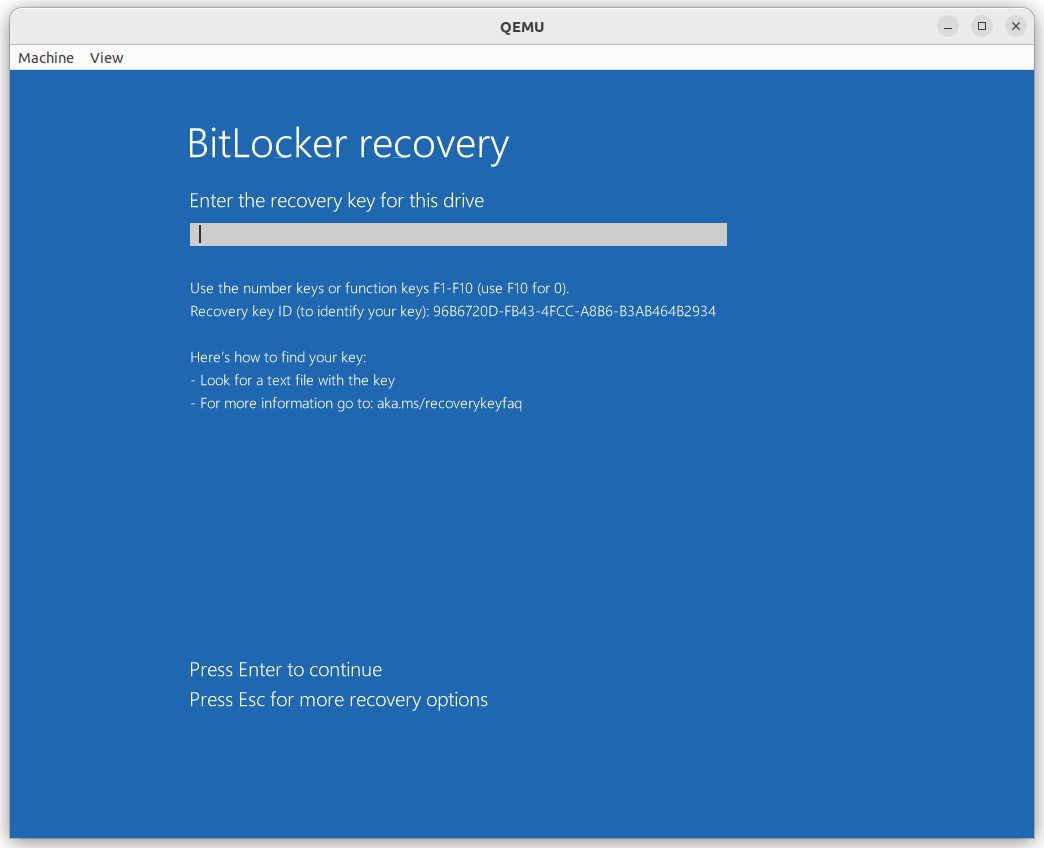
\includegraphics[width=\textwidth]{attacks/bitlocker/01_recovery_prompt.png}

% tpm values different
This happens due to TPM PCR values differing from what was initially used to seal the VMK, leaving the Windows bootloader unable to retrieve an unencrypted VMK from the TPM and as a result unable to decrypt the Windows installation. \TODO{the two different bitlocker volumes}

% bitlocker auto decryption fails
% boot execution differs from executing rootkit
\TODO{which measurements are used for sealing and unsealing}
\TODO{which ones are altered by the rootkit being present}


In theory this is as far as we get, BitLocker in combination of TPM measurements successfully mitigates UEFI attacks by disovering a deviation in the boot flow.
% what is the reaction of the average user
In practice we have to ask ourselves the question how a user reacts to seeing the BitLocker recovery prompt and the consequences to the action the user takes. As an immediate reaction the user has two options: entering the recovery key into the prompt or not entering the recovery key.
% motivation behind user decision
What decision the user makes is dependent on their tech saviness and influenced by a variety of factors such as urgency of booting into Windows, knowing alternatives to what the prompt tells them.
It is reasonable to assume that the average user is willingly entering their recovery key in response to the prompt as the prompt does not suggest any malicious causes or any negative reprocussions in following the instructions. The link mentioned in the prompt also only aids in locating the reocvery key \cite{microsoft-recovery-key-faq}.
\TODO{mention microsofts reasons for the prompt to be triggered}
\TODO{what is the actual alternative}
% does the user trust the system
% why would they not trust the system
% (ask admin for recovery password)
% type in recovery password
% alternative would be to remove drive and insert into safe device

Having the user enter their recovery key does not directly benefit our endevaours as BitLocker does not en/decrypt the hard drive as a whole upon boot but instead performs these respective action when reading or writing a block of data to or from the hard drive.

What we can do is try to record the keystrokes performed by the user while entering their recovery key and use it at some later point to gain control over the hard drive. A program designed to perform this type of attack is called a keylogger.

To implement such a keylogger we have to alter the code execution that happens when the recovery prompt is shown. For this our first step is to find our what execution environment or UEFI stage we are in, is Windows already using separate drivers for keyboard access or still relying on the UEFI environment and its protocols.

% ref to background os loader
% prompt is done by the OS Loader
% ergo still during transient system load phase
% required to use protocol services
% therefor uses uefi services for IO
% such as SimpleTextInputEx Protocol
% go over the two different input protocols
% find out which one is used
The UEFI specification defines two protocols which are used to abstract keyboard input these are the \lstinline{{SimpleTextInputProtocol} and the \lstinline{{SimpleTextInputExProtocol} \cite[12.2, 12.3]{uefi-spec}. To figure out if the recovery prompt uses these to read key strokes we can just add some print statements to the \lstinline{ReadKeyStroke} and \lstinline{ReadKeyStrokeEx} functions of their implementations in the edk2 OVMF package. On the next boot when typing we find that our \lstinline{ReadKeyStrokeEx} print statements from the \lstinline{{SimpleTextInputExProtocol} are triggered.

Now, knowing that the BitLocker recovery prompt is shown by an application running in the UEFI boottime environment, we can leverage this environment to implement our keylogger.

% explain more in depth how protocols are returned to the end user
% one instance per controller/handle
\TODO{how are protocols returned to the end user}
% explain basic back to the caller. This method is called function hooking
% explain how we retain information of the hook in question
% map protocol pointer to hook information
% keylog recovery key
To alter the code execution when performing a key stroke we can just iterate over all instances of the \lstinline{{SimpleTextInputExProtocol} and reassign the \lstinline{ReadKeyStrokeEx} entry of the struct, which is a function pointer. We will save each protocol instances' original function address and instead have it point to an intermediary function. This intermediary calls the original function and performs logging of the key stroke result before relaying the result to the caller. This method is called function hooking and is intransparent to consumer of a protocol.

%  show whole protocol
% WaitForKeyEx event
% wait for event
% query which key it was

\TODO{how is the SimpleTextInputEx Protocol used}

So far we are able to track each keystroke that queried via the \lstinline{ReadKeyStrokeEx} function, which in our testing is only done during the recovery prompt, but may be used by BIOS interactive menu.

\TODO{key input advancment is weird and makes tracking tricky}
F keys
block validity
only divisable by 11
cursor can move out of incomplete or valid blocks
up and down increments or decrements the cursor position

alternatively screen shot
still need hook to find when enter is pressed
explain how screenshotting works
some basic compression
wait for recovery key
send recovery key on enter press

on real hardware
network stack wasn't installed onto handles when boot over ip was disabled
compared loaded dxe drivers between both configurations with efi shell
Realtek Family driver not loaded
load manually
reinstall all handle to controllers to enable network stack regardless

sending key out is only good for physical access attack vector
dislocker linux utility
\cite{dislocker}
mount encrypted drive with decryption mean
read and write access
dual boot in vm
enter recovery key and it works
port to uefi

bitlocker encrypts block-wise

% blk and fs
\TODO{explain block devices}
\TODO{explain file system indepent abstraction better}
uefi protocol stack
\TODO{diagram of block io, disk io, simple filesystem and file protocol interaction (with hindsight of adding dislocker beneath block io)}
\cite[13.3.2 Partition Disocvery]{uefi-spec}
Drivers providing Simple File System Protocol use the Block I/O Protocol to access the underlying media.


hook block io
again hook data mapping

% execute after NTFS driver by doing it in an ExitBootServices hook
It is beneficial for us to write our payload to the Windows installation as close to the end of the UEFI environment as possible, this will maximize the presence of drivers and their offered access to hardware devices. It is also a wise design decision for the attacks following to this one. The call of the function \lstinline{ExitBootServices} marks the point of transitioning from boot time to runtime where the operating system takes over the control of the system, it presents a good opportunity for us to perform the write action of our rootkit.
% was muss man beachten bei exitbootservices hooking
\cite{exitbootservices-hooking}
hook ExitBootServices
enable hook
write payload
import registry key
disable hook

next boot would require to recovery key again
% https://learn.microsoft.com/en-us/windows/security/information-protection/bitlocker/bitlocker-use-bitlocker-drive-encryption-tools-to-manage-bitlocker
update tpm values in payload
caveat pin? look into this

% reference to rootkit definition
persistence when part of root of trust
fresh install / tpm update values
% paper von betreuern
hook Trusted Copmuting Group 2 (TCG2) Protocol
TPM communication
\cite[6.7.3]{tcg-efi-platform-spec}
% \cite[12.7 TPM_Unseal]{tcg-tpm-library-part3-commands}
receive bitlocker vmk key and send to dislocker

% https://labs.withsecure.com/publications/sniff-there-leaks-my-bitlocker-key
% !TeX root = ../thesis.tex

% https://www.scribbr.com/research-paper/discussion/

% meaning, importance, and relevance of your results
% explaining and evaluating what you found, showing how it relates to your literature review

\chapter{Discussion}


Our attacks show, the differences between \ac{UEFI} firmware rootkits and \ac{UEFI} bootkits.


% bootkit vs rootkit
bootkit much easier
usb stick, from windows
windows installer
if no password present we can disable secure boot
in case of physical presence it may require to change boot order
physical presence with bootable usb stick (defeated by secure boot)
genrally defeated by secure boot where as the rootkit isnt
even if secure boot was implemented for FV images, it could be patched if the validation change starts within the image

barrier of entry is higher
exploit to overwrite spi flash or be delivered with supply chain difficult
physical presence remove spi chip and emulate spi chip or modify chip content
but high payoff with persistence

% persistence
bootkit moves with hard drive but can be overwritten by fresh install
rootkit persistence across reinstallations or hard drive replacements


% SMM rootkit very powerful, complete control over the system
% \cite{}  https://pdfs.semanticscholar.org/68e7/42523f493b78111031a5a221a8cf767064f4.pdf

% attack assumption reflected to real world aplicability
didnt prevent firmware update overwriting our payload
generally the bitlocker reocvery prompt can raise suspicion and may lead to investigations and the threat to be found
BitLogger is more of a last resort and a social engineering aspect comparable to phishing
implications of windows secure boot PCR7 binding and use of secure boot system integrity check and validation profile 7, 11 is a bad decision of microsoft, that for example allows stolen laptops to be unlocked when infecting the firmware with our rootkit

it is generally very easy to attack windows from the \ac{UEFI} environment and there is little that they can do, as especially all windows code can be patched


\section{Mitigations}

bios password against secure boot removal or bootkit installation from USB

windows cant assume what the implementation of ReadKeyStrokeEx looks like (normally function patching might have a jump etc, which we dont even have here)

hardware validated boot to start the validation change from outside the image

inaccessible spi flash

tpm + pin/usb detectability

\subsection{User awareness}

% https://learn.microsoft.com/en-us/windows/security/information-protection/bitlocker/bitlocker-group-policy-settings#configure-the-pre-boot-recovery-message-and-url
% https://learn.microsoft.com/en-us/windows/security/information-protection/bitlocker/bcd-settings-and-bitlocker
you can change recovery message and URL in BCD hive


% https://learn.microsoft.com/en-us/windows/security/information-protection/bitlocker/bitlocker-recovery-guide-plan

recovery guide

what causes bitlocker recovery
- password wrong too often
- TPM 1.2, changing the BIOS or firmware boot device order
- Having the CD or DVD drive before the hard drive in the BIOS boot order and then inserting or removing a CD or DVD
- Failing to boot from a network drive before booting from the hard drive.
- Docking or undocking a portable computer
- Changes to the NTFS partition table on the disk including creating, deleting, or resizing a primary partition.
- Entering the personal identification number (PIN) incorrectly too many times
- Upgrading critical early startup components, such as a BIOS or UEFI firmware upgrade
- Updating option ROM firmware graphics card
- Adding or removing hardware
- REMOVING, INSERTING, OR COMPLETELY DEPLETING THE CHARGE ON A SMART BATTERY ON A PORTABLE COMPUTER
- Pressing the F8 or F10 key during the boot process
what does the recovery screen say \autoref{fig:bitlocker-recovery-prompt}

% https://learn.microsoft.com/en-us/windows/security/information-protection/bitlocker/bitlocker-device-encryption-overview-windows-10
% https://learn.microsoft.com/en-us/mem/configmgr/protect/deploy-use/bitlocker/helpdesk-portal?source=recommendations
% https://learn.microsoft.com/en-us/microsoft-desktop-optimization-pack/mbam-v25/
Enables end users to recover encrypted devices independently by using the Self-Service Portal

googeln wie legitime recovery key prompt reaktion aussieht

enterprise policy recovery key einschraenkbar?

enterprise policy on recovery key loss

vermitteln was das prompt bedeuten koennte

aber kann man einfach nicht anzeigen lassen

Security Flaw of entering a Recovery Password in an inheritly unsafe System

enterprise doesnt hand out recovery keys and instead receives hard drive


!!!!!!!!!!!!!!!!!!!!!!!!!
without hardware chain of trust a compromised system can patch/change any software and fixes are impossible

phishing prompts on their own
% !TeX root = ../thesis.tex

\chapter{Conclusion}
\label{sec:conclusion}

Our practical analysis of \ac{UEFI} threats against Windows 11 showed that enabling Secure Boot when using BitLocker comes with a hidden reduction in security.
Microsoft misuses Secure Boot in an attempt to provide platform firmware integrity validation, where the \ac{TPM} already offers a perfectly fine solution.
With such a misconfigured BitLocker validation profile our rootkit was able to sniff the communication between the Windows Boot Manager and \ac{TPM} without introducing side effects.
Through interception of the \emph{unseal} command, we gained access to the unencrypted BitLocker \ac{VMK}, to decrypt the hard drive and deploy further payload in the Windows installation.
By then modifying the Windows registry our payload was executed with privileges of the local system account.

Microsoft also has set a dangerous precedent by offering the user a mechanism to override the security reaction to integrity violations in an inherently untrustworthy system.
In the case of a correctly configured BitLocker validation profile, the code of our root- or bootkit measured into the \ac{TPM} cause the \emph{unseal} operation to fail and the Windows Boot Manager to trigger a recovery prompt.
The burden of security enforcement is now left to the user and when they decide to put further trust into the system and enter their recovery key, our \emph{BitLogger} can record the performed keystrokes to decrypt the hard drive.

\section*{Future Work}

It would be interesting to take a closer look at memory\-/based attacks under the light of \ac{VBS} like \ac{HVCI} and how rootkits might interact with the \ac{SMM} to circumvent these security mechanisms.
Further investigations into platforms where the \ac{RTM} is being established by the \ac{SRTM} measuring itself, could reveal these implementations to be much more vulnerable against rootkits than laid out in this thesis.
Verifying whether the current implementations of \ac{HVB} provide a gapless security chain might be of similar interest.


% --------------------------
% Back matter
% --------------------------
%
{%
    \setstretch{1.1}
    \renewcommand{\bibfont}{\normalfont\small}
    \setlength{\biblabelsep}{0pt}
    \setlength{\bibitemsep}{0.5\baselineskip plus 0.5\baselineskip}
    \printbibliography[nottype=online]
    \newrefcontext[labelprefix={@}]
    \printbibliography[heading=subbibliography,title={Webpages},type=online]
}
\cleardoublepage

\listoffigures
\cleardoublepage

\listoftables
\cleardoublepage

\lstlistoflistings
\cleardoublepage

\appendix\cleardoublepage
% !TEX root = ../thesis.tex

\chapter{Appendix}

\section{System Table}
\lstinputlisting[language=C,caption={System Table},captionpos=b,label=lst:system-table]{code/system_table.h}
\clearpage

\subsection{Boot Services}
\lstinputlisting[language=C,caption={Boot Services},captionpos=b,label=lst:boot-services]{code/boot_services.h}
\clearpage

\subsection{Runtime Services}
\lstinputlisting[language=C,caption={Runtime Services},captionpos=b,label=lst:runtime-services]{code/runtime_services.h}
\clearpage

\section{Protocols}

\subsection{Loaded Image Protocol}
\lstinputlisting[language=C,firstline=4,caption={Loaded Image Protocol},captionpos=b,label=lst:loaded-image-protocol]{code/protocols/LoadedImage.h}

\clearpage

\subsection{Driver Binding Protocol}
\lstinputlisting[language=C,firstline=4,caption={Driver Binding Protocol},captionpos=b,label=lst:driver-binding-protocol]{code/protocols/DriverBinding.h}

\clearpage

\subsection{Simple File System and File Protocol}
\lstinputlisting[language=C,firstline=4,caption={Simple File System and File Protocol},captionpos=b,label=lst:simple-file-system-protocol]{code/protocols/SimpleFileSystem.h}

\clearpage

\subsection{Disk \acs{I/O} Protocol}
\lstinputlisting[language=C,firstline=4,caption={Disk \ac{I/O} Protocol},captionpos=b,label=lst:disk-io-protocol]{code/protocols/DiskIo.h}

\clearpage

\subsection{Block \acs{I/O} Protocol}
\lstinputlisting[language=C,firstline=4,caption={Block \ac{I/O} Protocol},captionpos=b,label=lst:block-io-protocol]{code/protocols/BlockIo.h}

\clearpage

\subsection{\acf{BDS} Protocol}

\lstinputlisting[language=C,firstline=4,caption={\ac{BDS} Protocol},captionpos=b,label=lst:tcg2-protocol]{code/protocols/Bds.h}

\clearpage

\subsection{Firmware Volume2 Protocol}

\lstinputlisting[language=C,firstline=4,caption={\ac{BDS} Protocol},captionpos=b,label=lst:firmware-volume2-protocol]{code/protocols/FirmwareVolume2.h}

\clearpage

\subsection{Simple Text Input Protocol}
\lstinputlisting[language=C,firstline=4,caption={Simple Text Input Ex Protocol},captionpos=b,label=lst:simple-text-input-protocol]{code/protocols/SimpleTextIn.h}

\clearpage

\subsection{Simple Text Input Ex Protocol}
\lstinputlisting[language=C,firstline=4,caption={Simple Text Input Ex Protocol},captionpos=b,label=lst:simple-text-input-ex-protocol]{code/protocols/SimpleTextInEx.h}

\clearpage

\subsection{\acs{TCG}2 Protocol}
\lstinputlisting[language=C,firstline=4,caption={\ac{TCG}2 Protocol},captionpos=b,label=lst:tcg2-protocol]{code/protocols/Tcg2Protocol.h}

\clearpage


\section{Firmware File Types}

\begin{table}[htb]
    \label{tab:file-types}
    \centering
    \small
    \begin{tabularx}{1.05\textwidth}{XcX}
        \toprule
        \textbf{Name}                                                                  & \textbf{Value}          & \textbf{Description}                                                                                                        \\
        \midrule
        \code{EFI\_FV\_FILETYPE\_RAW}                                                  & \code{0x01}             & Binary data                                                                                                                 \\
        \arrayrulecolor{gray}
        \midrule[0.3pt]
        \code{EFI\_FV\_FILETYPE\_FREEFORM}                                             & \code{0x02}             & Sectioned data                                                                                                              \\
        \midrule[0.3pt]
        \code{EFI\_FV\_FILETYPE\_SECURITY\_CORE}                                       & \code{0x03}             & Platform core code used during the SEC phase                                                                                \\
        \midrule[0.3pt]
        \code{EFI\_FV\_FILETYPE\_PEI\_CORE}                                            & \code{0x04}             & PEI Foundation                                                                                                              \\
        \midrule[0.3pt]
        \code{EFI\_FV\_FILETYPE\_DXE\_CORE}                                            & \code{0x05}             & DXE Foundation                                                                                                              \\
        \midrule[0.3pt]
        \code{EFI\_FV\_FILETYPE\_PEIM}                                                 & \code{0x06}             & PEI module (PEIM)                                                                                                           \\
        \midrule[0.3pt]
        \code{EFI\_FV\_FILETYPE\_DRIVER}                                               & \code{0x07}             & DXE driver                                                                                                                  \\
        \midrule[0.3pt]
        \code{EFI\_FV\_FILETYPE\_COMBINED\_PEIM\_DRIVER}                               & \code{0x08}             & Combined PEIM/DXE driver                                                                                                    \\
        \midrule[0.3pt]
        \code{EFI\_FV\_FILETYPE\_APPLICATION}                                          & \code{0x09}             & Application                                                                                                                 \\
        \midrule[0.3pt]
        \code{EFI\_FV\_FILETYPE\_MM}                                                   & \code{0x0A}             & Contains a PE32+ image that will be loaded into MMRAM in MM Traditional Mode.                                               \\
        \midrule[0.3pt]
        \code{EFI\_FV\_FILETYPE\_FIRMWARE\_VOLUME\_IMAGE}                              & \code{0x0B}             & Firmware volume image                                                                                                       \\
        \midrule[0.3pt]
        \code{EFI\_FV\_FILETYPE\_COMBINED\_MM\_DXE}                                    & \code{0x0C}             & Contains PE32+ image that will be dispatched by the DXE Dispatcher and will also be loaded into MMRAM in MM Tradition Mode. \\
        \midrule[0.3pt]
        \code{EFI\_FV\_FILETYPE\_MM\_CORE}                                             & \code{0x0D}             & MM Foundation that support MM Traditional Mode.                                                                             \\
        \midrule[0.3pt]
        \code{EFI\_FV\_FILETYPE\_MM\_STANDALONE}                                       & \code{0x0E}             & Contains a PE32+ image that will be loaded into MMRAM in MM Standalone Mode.                                                \\
        \midrule[0.3pt]
        \code{EFI\_FV\_FILETYPE\_MM\_CORE\_STANDALONE}                                 & \code{0x0F}             & MM Foundation that support MM Tradition Mode and MM Standalone Mode.                                                        \\
        \midrule[0.3pt]
        \code{EFI\_FV\_FILETYPE\_OEM\_MIN\dots} \code{EFI\_FV\_FILETYPE\_OEM\_MAX}     & \code{0xC0}-\code{0xDF} & OEM File Types                                                                                                              \\
        \midrule[0.3pt]
        \code{EFI\_FV\_FILETYPE\_DEBUG\_MIN\dots} \code{EFI\_FV\_FILETYPE\_DEBUG\_MAX} & \code{0xE0}-\code{0xEF} & Debug/Test File Types                                                                                                       \\
        \midrule[0.3pt]
        \code{EFI\_FV\_FILETYPE\_FFS\_MIN\dots} \code{EFI\_FV\_FILETYPE\_FFS\_MAX}     & \code{0xF0}-\code{0xFF} & Firmware File System Specific File Types                                                                                    \\
        \midrule[0.3pt]
        \code{EFI\_FV\_FILETYPE\_FFS\_PAD}                                             & \code{0xF0}             & Pad File For FFS                                                                                                            \\
        \arrayrulecolor{black}
        \bottomrule
    \end{tabularx}
    \caption{Firmware File Types \cite[Vol. 3, Table 3-3]{pi-spec}}

    \normalsize
\end{table}

\clearpage

\section{Firmware File Section Types}

\begin{table}[htb]
    \label{tab:file-section-types}
    \centering
    \small
    \begin{tabularx}{1.0\textwidth}{XcX}
        \toprule
        \textbf{Name}                               & \textbf{Value} & \textbf{Description}                                                                                                                                    \\
        \midrule
        \code{EFI\_SECTION\_COMPRESSION}            & \code{0x01}    & Encapsulation section where other sections are compressed.                                                                                              \\
        \arrayrulecolor{gray}
        \midrule[0.3pt]
        \code{EFI\_SECTION\_GUID\_DEFINED}          & \code{0x02}    & Encapsulation section where other sections have format defined by a \acs{GUID}.                                                                         \\
        \midrule[0.3pt]
        \code{EFI\_SECTION\_DISPOSABLE}             & \code{0x03}    & Encapsulation section used during the build process but not required for execution.                                                                     \\
        \midrule[0.3pt]
        \code{EFI\_SECTION\_PE32}                   & \code{0x10}    & PE32+ Executable image.                                                                                                                                 \\
        \midrule[0.3pt]
        \code{EFI\_SECTION\_PIC}                    & \code{0x11}    & Position-Independent Code.                                                                                                                              \\
        \midrule[0.3pt]
        \code{EFI\_SECTION\_TE}                     & \code{0x12}    & Terse Executable image.                                                                                                                                 \\
        \midrule[0.3pt]
        \code{EFI\_SECTION\_DXE\_DEPEX}             & \code{0x13}    & DXE Dependency Expression.                                                                                                                              \\
        \midrule[0.3pt]
        \code{EFI\_SECTION\_VERSION}                & \code{0x14}    & Version, Text and Numeric.                                                                                                                              \\
        \midrule[0.3pt]
        \code{EFI\_SECTION\_USER\_INTERFACE}        & \code{0x15}    & User-Friendly name of the driver.                                                                                                                       \\
        \midrule[0.3pt]
        \code{EFI\_SECTION\_COMPATIBILITY16}        & \code{0x16}    & DOS-style 16-bit EXE.                                                                                                                                   \\
        \midrule[0.3pt]
        \code{EFI\_SECTION\_FIRMWARE\_VOLUME\_IMAG} & \code{0x17}    & PI Firmware Volume image.                                                                                                                               \\
        \midrule[0.3pt]
        \code{EFI\_SECTION\_FREEFORM\_SUBTYPE\_GUI} & \code{0x18}    & Raw data with GUID in header to define format.                                                                                                          \\
        \midrule[0.3pt]
        \code{EFI\_SECTION\_RAW}                    & \code{0x19}    & Raw data.                                                                                                                                               \\
        \midrule[0.3pt]
        \code{EFI\_SECTION\_PEI\_DEPEX}             & \code{0x1B}    & PEI Dependency Expression.                                                                                                                              \\
        \midrule[0.3pt]
        \code{EFI\_SECTION\_MM\_DEPEX}              & \code{0x1C}    & Leaf section type for determining the dispatch order for an MM Traditional driver in MM Traditional Mode or MM Standalone driver in MM Standalone Mode. \\
        \arrayrulecolor{black}
        \bottomrule
    \end{tabularx}
    \caption{Firmware File Section Types \cite[Vol. 3, Table 3-4]{pi-spec}}
    \normalsize
\end{table}
       % INCLUDE: appendix

\cleardoublepage
% !TEX root = ../thesis.tex

\chapter*{List of Acronyms}
\label{sec:acronyms}

\begin{acronym}[DEPEX]
    \acro{ACPI}{Advanced Configuration and Power Interface}%
    \acro{AES}{Advanced Encryption Standard}%
    \acro{AL}{Afterlife}%
    \acro{API}{Application Programming Interface}%
    \acro{ASCII}{American Standard Code for Information Interchange}%
    \acro{BCD}{Boot Configuration Data}%
    \acro{BDE}{BitLocker Drive Encryption}%
    \acro{BDS}{Boot Device Selection}%
    \acro{BF}{Boot Firmware}%
    \acro{BFV}{\acl{BF} Volume}%
    \acro{BIOS}{Basic \acl{I/O} System}%
    \acro{CA}{Certificate Authority}%
    \acro{CAR}{Cache as \acl{RAM}}%
    \acro{CD}{Compact Disc}%
    \acro{CRTM}{Core \acl{RTM}}%
    \acro{CSM}{Compatibility Support Module}%
    \acro{CPU}{Central Processing Unit}%
    \acro{DB}{Data Base}%
    \acro{DEPEX}{Dependency Expression}%
    \acro{DLL}{Dynamically Linked Library}%
    \acro{DXE}{Driver Execution Environment}%
    \acro{EDK}{\acs{EFI} Development Kit}%
    \acro{EFI}{Extensible Firmware Interface}%
    \acro{ELAM}{Early-Launch Antimalware}%
    \acro{ESP}{\acs{EFI} System Partition}%
    \acro{FAT}{File Allocation Table}%
    \acro{FD}{Firmware Device}%
    \acro{FDF}{Flash Description File}%
    \acro{FFS}{Firmware Filesystem}%
    \acro{FUSE}{Filesystem in Userspace}%
    \acro{FV}{Firmware Volume}%
    \acro{FVE}{Full Volume Encryption}%
    \acro{FVEK}{\acl{FVE} Key}%
    \acro{GPT}{\acs{GUID} Partition Table}%
    \acro{GUID}{Globally Unique Identifier}%
    \acro{HOB}{Hand-off Block}%
    \acro{H-CRTM}{Hardware-\acl{CRTM}}%
    \acro{I/O}{Input/Output}%
    \acro{IBB}{Initial Boot Block}%
    \acro{KEK}{Key Exchange Key}%
    \acro{LBA}{Logical Block Address}%
    \acro{LPC}{Low Pin Count}%
    \acro{MBR}{Master Boot Record}%
    \acro{NTFS}{New Technology File System}%
    \acro{NVRAM}{Non\-/volatile \acs{RAM}}%
    \acro{OEM}{Original Equipment Manufacturer}%
    \acro{OS}{Operating System}%
    \acro{OVMF}{Open Virtual Machine Firmware}%
    \acro{PC}{Personal Computer}%
    \acro{PCI}{Peripheral Component Interconnect}%
    \acro{PCR}{Platform Configuration Register}%
    \acro{PE32}{Portable Executable 32-Bit}%
    \acro{PEI}{Pre-\acs{EFI} Initialization}%
    \acro{PEIM}{\acl{PEI} Module}%
    \acro{PF}{Platform Firmware}%
    \acro{PI}{Platform Initialization}%
    \acro{PIN}{Personal Identification Number}%
    \acro{PK}{Platform Key}%
    \acro{PPI}{\acs{PEIM}-to-\acs{PEIM} Interface}%
    \acro{QEMU}{Quick Emulator}%
    \acro{RAM}{Random Access Memory}%
    \acro{ROM}{Read-Only Memory}%
    \acro{RT}{Runtime}%
    \acro{RTM}{Root of Trust for Measurement}%
    \acro{RTM}{Root of Trust for Storage}%
    \acro{SEC}{Security}%
    \acro{SMM}{System Management Mode}%
    \acro{SRTM}{Static Root of Trust for Measurement}%
    \acro{SPI}{Serial Peripheral Interface}%
    \acro{TB}{Terra Byte}%
    \acro{TCG}{Trusted Computing Group}%
    \acro{TPM}{Trusted Platform Module}%
    \acro{TSL}{Transient System Load}%
    \acro{UEFI}{Unified \acl{EFI}}%
    \acro{USB}{Universal Serial Bus}%
    \acro{UUID}{Universally Unique Identifier}%
    \acro{VBR}{Volume Boot Record}%
    \acro{VMK}{Volume Master Key}%
    \acro{XML}{Extensible Markup Language}%
\end{acronym}
\clearpage

\newpage
\mbox{}

\end{document}